% !TeX root = report_scichal4A.tex

\documentclass[a4paper, 12pt]{article}
\usepackage[utf8]{inputenc}
\usepackage[portuguese]{babel}
\usepackage{hyperref} % insert url
\usepackage{booktabs} % fazer tabelas
\usepackage{mathptmx}
\usepackage{enumitem}
\usepackage{siunitx}

\usepackage{amsmath}

% Margins
\usepackage{geometry}
\geometry{left=30mm,right=20mm, bindingoffset=0mm, top=30mm,bottom=20mm,includefoot}

% Images
\usepackage{graphicx}
\graphicspath{ {./images/} }
\usepackage{subcaption}

% Indent first sentence of a paragraph
\usepackage{indentfirst}

% Page numbers at bottom right
\usepackage{fancyhdr}
\pagestyle{fancy}
\fancyhf{}
\renewcommand{\headrulewidth}{0pt}
\rfoot{\thepage}

% 1.5 line spacing (yes, 1.25 is actually 1.5)
\fontsize{10}{12}
\linespread{1.50}
\fontfamily{ptm}
\selectfont

% Indent size
\setlength\parindent{10mm}

% Jump 20pt
\newcommand{\jump}[1]{{\vspace{20pt}}}

% Summary
\usepackage{tocloft}
\renewcommand{\cftsecfont}{\bfseries}  % Seções em negrito
\renewcommand{\cftsecpagefont}{\bfseries} % Números de página em negrito
\setlength{\cftbeforesecskip}{0.5cm} % Espaçamento entre seções no sumário
\usepackage{multirow}

% Page numbers at bottom right, and dynamic section name at bottom left
\usepackage{fancyhdr}
\pagestyle{fancy}
\fancyhf{}
\renewcommand{\headrulewidth}{0pt}
\fancyfoot[L]{\nouppercase{\leftmark}} % Adds the name of the current section to the left corner of the footer
\fancyfoot[R]{\thepage} % Page number in the right corner of the footer
\renewcommand{\footrulewidth}{0.4pt} % Sets a thin line in the footer

% Footer spacing
\usepackage[bottom]{footmisc}
\setlength{\footskip}{50pt} % Adjust the value as needed.

%% Code style
\usepackage{listings} % package to put code line
\usepackage{float}
\usepackage{xcolor,enumerate}

\definecolor{codegreen}{rgb}{0,0.6,0}
\definecolor{codegray}{rgb}{0.5,0.5,0.5}
\definecolor{codepurple}{rgb}{0.58,0,0.82}
\definecolor{backcolour}{rgb}{0.95,0.95,0.92}

\lstdefinestyle{mystyle}{
    backgroundcolor=\color{backcolour},   
    commentstyle=\color{codegreen},
    keywordstyle=\color{magenta},
    numberstyle=\tiny\color{codegray},
    stringstyle=\color{codepurple},
    basicstyle=\ttfamily\footnotesize,
    breakatwhitespace=false,         
    breaklines=true,                 
    captionpos=b,                    
    keepspaces=true,                 
    numbers=left,                    
    numbersep=5pt,                  
    showspaces=false,                
    showstringspaces=false,
    showtabs=false,                  
    tabsize=2,
    literate=
        {á}{{\'a}}1
        {à}{{\`a}}1
        {ã}{{\~a}}1
        {â}{{\^a}}1
        {é}{{\'e}}1
        {ê}{{\^e}}1
        {ê}{{\^e}}1
        {í}{{\'i}}1
        {ó}{{\'o}}1
        {õ}{{\~o}}1
        {ú}{{\'u}}1
        {ü}{{\"u}}1
        {ç}{{\c{c}}}1
}

\lstset{style=mystyle}

\newenvironment{leftquote}[1][]
{
    \hspace{30pt} #1
    \vspace{20pt}
    \fontsize{10}{10}\selectfont
    \begin{flushright}
    \begin{minipage}{120mm}
}
{
    \end{minipage}
    \end{flushright}
    \par
    \vspace{20pt}
}

\newcommand{\tmp}{}

\newenvironment{container}[3]
{
    \renewcommand{\tmp}{#3} %gambiarra
    
    \begin{center}
    \begin{minipage}{#1}
    \centering
    #2
}
{
    \raggedright
    {\footnotesize \tmp}
    \end{minipage}
    \end{center}
}
\usepackage{amsmath, amssymb}
\usepackage{pgfplots}
\pgfplotsset{compat=1.18}
\usepackage{tikz}
\usetikzlibrary{arrows.meta}
\usetikzlibrary{arrows.meta}

\bibliographystyle{ieeetr} % Estilo de citação


\begin{document}
% LTeX: language=pt-BR
% ------------------------------------------------------ %
% ----------------- Capa do Trabalho ------------------- %

\clearpage
\thispagestyle{empty}

\begin{bfseries}
\begin{center}


\includegraphics[scale=0.45]{Imagens/ufc.png} \\
\vspace{-4pt} 
UNIVERSIDADE FEDERAL DO CEARÁ \\
\vspace{4pt} 
CENTRO DE TECNOLOGIA \\
\vspace{4pt} 
DEPARTAMENTO DE TELEINFORMÁTICA \\
\vspace{4pt}
COEXISTÊNCIA E COMPARTILHAMENTO DINÂMICO DE ESPECTRO EM COMUNICAÇÕES MÓVEIS 6G \\
\vspace{4pt}

\vspace*{\fill}
\rule{\linewidth}{0.1mm}\\[0.7cm ]
{\Large\textbf{RELATÓRIO SCIENCE CHALENGE 4A}}\\[0.25cm]
\rule{\linewidth}{0.1mm} \\[1.0cm]

\textbf{PROFESSOR: F. RODRIGO P. CAVALCANTI}

\vspace*{\fill}

\end{center}

\begin{itemize}[leftmargin=*]
    \setlength{\itemsep}{0pt}
    \item[] MIKAEL RIBEIRO CAMELO - 509482
    \item[] CAIO RODRIGUES
\end{itemize}

\vspace*{\fill}

\begin{center}
    \textbf{FORTALEZA - CE}\\
    \textbf{2026.1}
\end{center}

\end{bfseries}

% --------------------------------------------- %
% ----------------- Sumário ------------------- %
\newpage
\tableofcontents
\newpage

% --------------------------------------------- %
% ------------- Lista de Siglas --------------- %
\section*{Lista de Siglas e Abreviaturas}
\addcontentsline{toc}{section}{Lista de Siglas e Abreviaturas}

\begin{itemize}[leftmargin=3cm, labelsep=0.5cm]
    \item[\textbf{AoA}] Ângulo de Chegada (\textit{Angle of Arrival})
    \item[\textbf{AP}] Ponto de Acesso (\textit{Access Point})
    \item[\textbf{CCI}] Interferência Co-canal (\textit{Co-Channel Interference})
    \item[\textbf{CDF}] Função Distribuição Acumulada (\textit{Cumulative Distribution Function})
    \item[\textbf{DPC}] Controle de Potência Distribuído (\textit{Distributed Power Control})
    \item[\textbf{EE}] Eficiência Energética (\textit{Energy Efficiency})
    \item[\textbf{KPI}] Indicador Chave de Desempenho (\textit{Key Performance Indicator})
    \item[\textbf{MIMO}] Múltiplas Entradas e Múltiplas Saídas (\textit{Multiple-Input Multiple-Output})
    \item[\textbf{MRC}] Combinação de Razão Máxima (\textit{Maximum Ratio Combining})
    \item[\textbf{PC}] Controle de Potência (\textit{Power Control})
    \item[\textbf{QAM}] Modulação de Amplitude em Quadratura (\textit{Quadrature Amplitude Modulation})
    \item[\textbf{QoS}] Qualidade de Serviço (\textit{Quality of Service})
    \item[\textbf{RRM}] Gerenciamento de Recursos de Rádio (\textit{Radio Resource Management})
    \item[\textbf{SE}] Eficiência Espectral (\textit{Spectral Efficiency})
    \item[\textbf{SINR}] Relação Sinal-Interferência mais Ruído (\textit{Signal-to-Interference-plus-Noise Ratio})
    \item[\textbf{SNR}] Relação Sinal-Ruído (\textit{Signal-to-Noise Ratio})
    \item[\textbf{UCA}] Arranjo Circular Uniforme (\textit{Uniform Circular Array})
    \item[\textbf{UE}] Equipamento do Usuário (\textit{User Equipment})
    \item[\textbf{ULA}] Arranjo Linear Uniforme (\textit{Uniform Linear Array})
\end{itemize}

\newpage

% --------------------------------------------- %
% ------------------ Seções ------------------- %
% --------------------------------------------- %
\section{Atividade 1: Otimização Conjunta Distribuída de \textit{Beamforming} e Controle de Potência}

Na primeira atividade é investigado o acoplamento entre a filtragem espacial via \textit{Adaptive Beamforming} com Combinação de Razão Máxima (MRC) e o Controle de Potência Distribuído (DPC) em uma topologia multicelular de $M = 16$ APs equipados com Arranjos Circulares Uniformes (UCA). O objetivo central consiste em maximizar a capacidade agregada da rede e a eficiência energética sem degradar a proteção conferida aos usuários de borda contra a Interferência Co-canal (CCI).

\subsection{Estratégia Distribuída \textit{Dual-Loop} e Negociação de Alvo}

O algoritmo de Controle de Potência Distribuído com alvo fixo (\textit{Fixed-Target DPC}) impõe uma meta única de SINR ($\gamma_{\text{tar}} = 10\text{ dB}$) a todos os terminais ativos. Embora essa abordagem reduza a interferência mútua, ela subutiliza o alto ganho direcional proporcionado pelo \textit{beamforming} adaptativo para usuários em condições favoráveis de propagação. Para superar essa limitação, implementou-se a arquitetura em malha dupla (\textit{Dual-Loop Distributed Strategy}):

\begin{itemize}
    \item \textbf{Malha Interna — Rápida:} Para cada usuário $k$, o algoritmo DPC atualiza iterativamente a potência de transmissão $p_k$ buscando convergir para a meta local instantânea $\gamma_{\text{tar},k}$.
    \item \textbf{Malha Externa — Lenta:} Ajusta dinamicamente o alvo $\gamma_{\text{tar},k}$ de cada terminal dentro da janela operacional de $[-10, 20]\text{ dB}$, partindo de um valor inicial de $10\text{ dB}$.
\end{itemize}

A estratégia de negociação de alvo (\textit{Target Negotiation}) no \textit{Outer Loop} segue três regras físicas associadas às limitações de potência e modulação:
\begin{itemize}
    \item \textbf{Aumento de Alvo:} Caso o UE atinja sua meta atual operando abaixo da potência máxima ($p_k < p_{\max}$), incrementa-se $\gamma_{\text{tar},k}$ em $+1\text{ dB}$ para explorar o ganho espacial do feixe MRC até o limite de saturação de $20\text{ dB}$ (imposto pelo teto das constelações QAM práticas).
    \item \textbf{Redução de Alvo:} Se o terminal saturar na potência máxima ($p_k = p_{\max} = 1\text{ W}$) e ainda assim não alcançar a meta ($\gamma_k < \gamma_{\text{tar},k}$), reduz-se $\gamma_{\text{tar},k}$ em $-1\text{ dB}$ para aliviar a interferência gerada sobre as células adjacentes.
    \item \textbf{Bloqueio de Terminal:} Caso o alvo negociado caia abaixo do limiar de sensibilidade de $-10\text{ dB}$ (ou se a SINR resultante ao final do processo permanecer inferior a $-10\text{ dB}$), o terminal desliga seu transmissor ($p_k = 0$) e entra em estado de \textit{Outage}.
\end{itemize}

Para garantir rigor estatístico e comparabilidade direta, o gerador de números pseudoaleatórios foi reinicializado com a mesma semente (\textit{seed}) antes da bateria de \textit{snapshots} de Monte Carlo de cada estratégia, assegurando realizações idênticas de posicionamento, sombreamento lognormal e desvanecimento rápido de Rayleigh.

\subsection{Análise Comparativa de KPIs (Exercício 1)}

A Tabela \ref{tab:act1_kpis} e a Figura \ref{fig:act1_bars} sintetizam o desempenho do esquema proposto (\textbf{Dual-Loop PC}) frente aos dois cenários de referência (\textbf{Full Power} a $1\text{ W}$ sem controle de potência e \textbf{DPC Fixo} com meta universal de $10\text{ dB}$) sob diferentes cargas de usuários por canal ($K \in \{1, 4, 8\}$).

\begin{table}[H]
    \centering
    \caption{Comparativo de KPIs para Joint MRC e Estratégias de Controle de Potência}
    \vspace{4pt}
    \resizebox{\textwidth}{!}{
        \begin{tabular}{c|l|cccc}
            \toprule
            \textbf{Carga ($K$)} & \textbf{Algoritmo} & \textbf{Border SE (10º Pct)} & \textbf{Sum-Capacity SE (Média)} & \textbf{Eficiência Energética} & \textbf{Taxa de Outage} \\
            & & \textbf{[bps/Hz]} & \textbf{[bps/Hz]} & \textbf{[Mbits/Joule]} & \textbf{[\%]} \\
            \midrule
            \multirow{3}{*}{$K = 1$} 
            & Full Power (1W)         & 1.05 & 3.84 & 384.03 & 0.26\% \\
            & DPC Fixo (Meta 10 dB)   & 1.05 & 2.77 & 446.89 & 0.26\% \\
            & Dual-Loop PC (Outage)   & 0.96 & 3.50 & \textbf{465.40} & 0.34\% \\
            \midrule
            \multirow{3}{*}{$K = 4$} 
            & Full Power (1W)         & 0.73 & 14.37 & 359.14 & 2.06\% \\
            & DPC Fixo (Meta 10 dB)   & \textbf{0.85} & 10.67 & 412.89 & \textbf{0.73\%} \\
            & Dual-Loop PC (Outage)   & 0.72 & 14.23 & \textbf{434.99} & 1.58\% \\
            \midrule
            \multirow{3}{*}{$K = 8$} 
            & Full Power (1W)         & 0.45 & 26.44 & 330.48 & 4.32\% \\
            & DPC Fixo (Meta 10 dB)   & \textbf{0.66} & 20.28 & 374.74 & \textbf{1.50\%} \\
            & Dual-Loop PC (Outage)   & 0.48 & \textbf{26.38} & \textbf{406.27} & 3.29\% \\
            \bottomrule
        \end{tabular}}
    \label{tab:act1_kpis}
\end{table}

\begin{figure}[H]
    \centering
    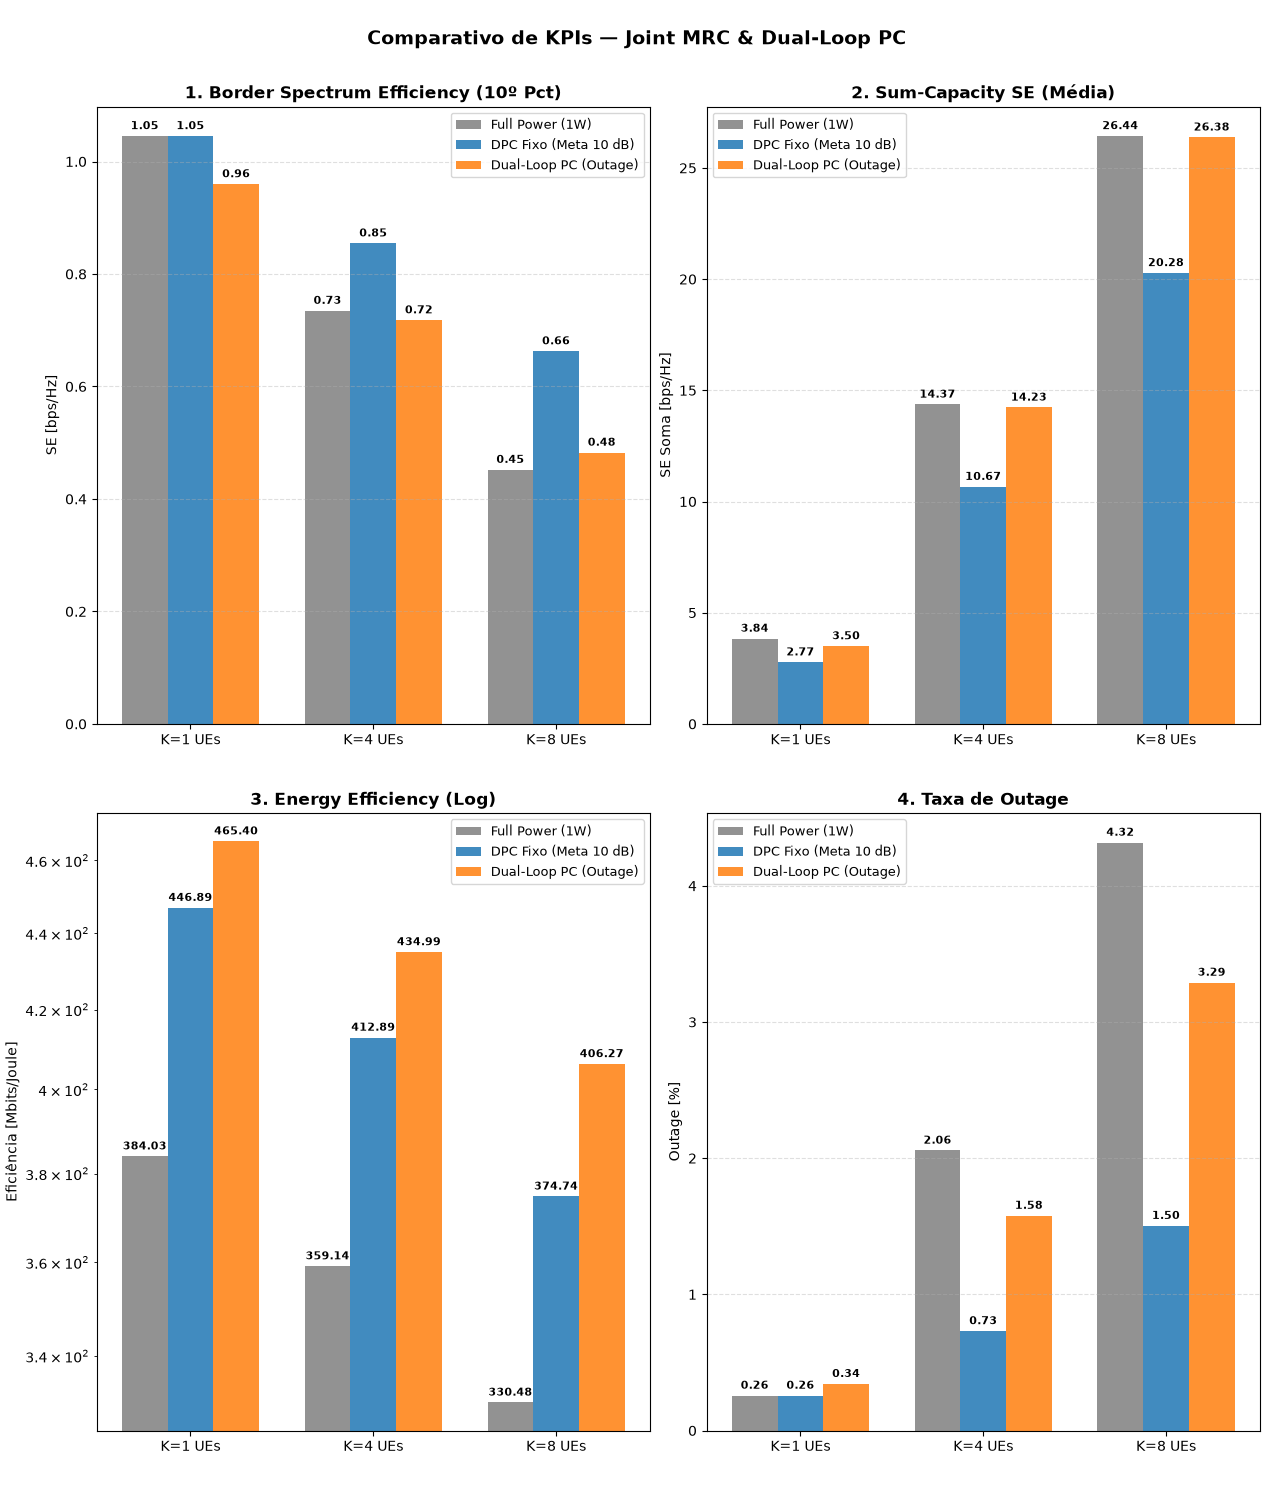
\includegraphics[width=0.95\linewidth]{Imagens/Activity01.png}
    \caption{Comparativo dos quatro KPIs primários para $K \in \{1, 4, 8\}$ UEs: (1) Eficiência Espectral de Borda no 10º percentil, (2) Eficiência Espectral de Capacidade Soma, (3) Eficiência Energética em escala logarítmica e (4) Taxa de Outage.}
    \label{fig:act1_bars}
\end{figure}

A análise conjunta dos indicadores revela o comportamento físico de cada política de alocação de potência:

\begin{itemize}
    \item \textbf{Recuperação da \textit{Sum-Capacity} e Ganho sobre o DPC Fixo:} O algoritmo de \textit{DPC Fixo (10 dB)} impõe um severo estrangulamento à vazão total da rede, reduzindo a \textit{Sum-Capacity SE} em $K=8$ de $26.44\text{ bps/Hz}$ para apenas $20.28\text{ bps/Hz}$ (uma perda de $23.3\%$) por proibir que usuários próximos aos APs aproveitem a diretividade do feixe MRC acima de $10\text{ dB}$. Em contrapartida, o \textbf{Dual-Loop PC} permite que enlaces fortes escalem suas metas até o teto de modulação de $20\text{ dB}$, alcançando $26.38\text{ bps/Hz}$ em $K=8$ — igualando a capacidade de topo da transmissão à plena potência (\textit{Full Power}).
    \item \textbf{Liderança Absoluta em Eficiência Energética:} Em todos os cenários de carga, o \textbf{Dual-Loop PC} atinge a maior Eficiência Energética da rede, entregando $465.40\text{ Mbits/Joule}$ ($K=1$), $434.99\text{ Mbits/Joule}$ ($K=4$) e $406.27\text{ Mbits/Joule}$ ($K=8$). Isso ocorre porque o \textit{Outer Loop} impede o desperdício de potência: assim que o UE atinge o limite de saturação de $20\text{ dB}$ da constelação QAM, qualquer potência adicional não se converte em taxa de dados útil, sendo poupada pelo algoritmo. Além disso, desligar terminais inviáveis (\textit{UE Blocking} abaixo de $-10\text{ dB}$) elimina o gasto energético de UEs que apenas gerariam interferência sem conseguir decodificar dados.
    \item \textbf{\textit{Trade-off} na Borda da Célula (\textit{Border SE} e \textit{Outage}):} Sob alta carga ($K=8$), o \textbf{Dual-Loop PC} supera a política \textit{Full Power} tanto na eficiência espectral de borda ($0.48\text{ bps/Hz}$ contra $0.45\text{ bps/Hz}$) quanto na redução da taxa de \textit{Outage} (caindo de $4.32\%$ para $3.29\%$), pois a contenção de potência dos UEs centrais reduz a interferência co-canal sobre as bordas. Observa-se que o \textit{DPC Fixo} obtém a maior \textit{Border SE} ($0.66\text{ bps/Hz}$) e o menor \textit{Outage} ($1.50\%$) em $K=8$ justamente por forçar todos os UEs centrais a operarem em níveis mínimos de potência, porém às custas de sacrificar quase um quarto da capacidade agregada do sistema. Nota-se ainda que, em $K=1$, a ligeira diferença na \textit{Border SE} do \textit{Dual-Loop} ($0.96\text{ bps/Hz}$ vs. $1.05\text{ bps/Hz}$) decorre da oscilação discreta de $\pm 1\text{ dB}$ do passo fixo da malha interna (\textit{UD-DPC}) quando o número de iterações internas é ímpar.
\end{itemize}

\subsection{Análise Estatística das CDFs (Potência, SINR e Capacidade)}

A Figura \ref{fig:act1_cdfs} apresenta as Funções Distribuição Acumulada (CDFs) da potência recebida, da SINR e da capacidade de canal para $K \in \{1, 4, 8\}$.

\begin{figure}[H]
    \centering
    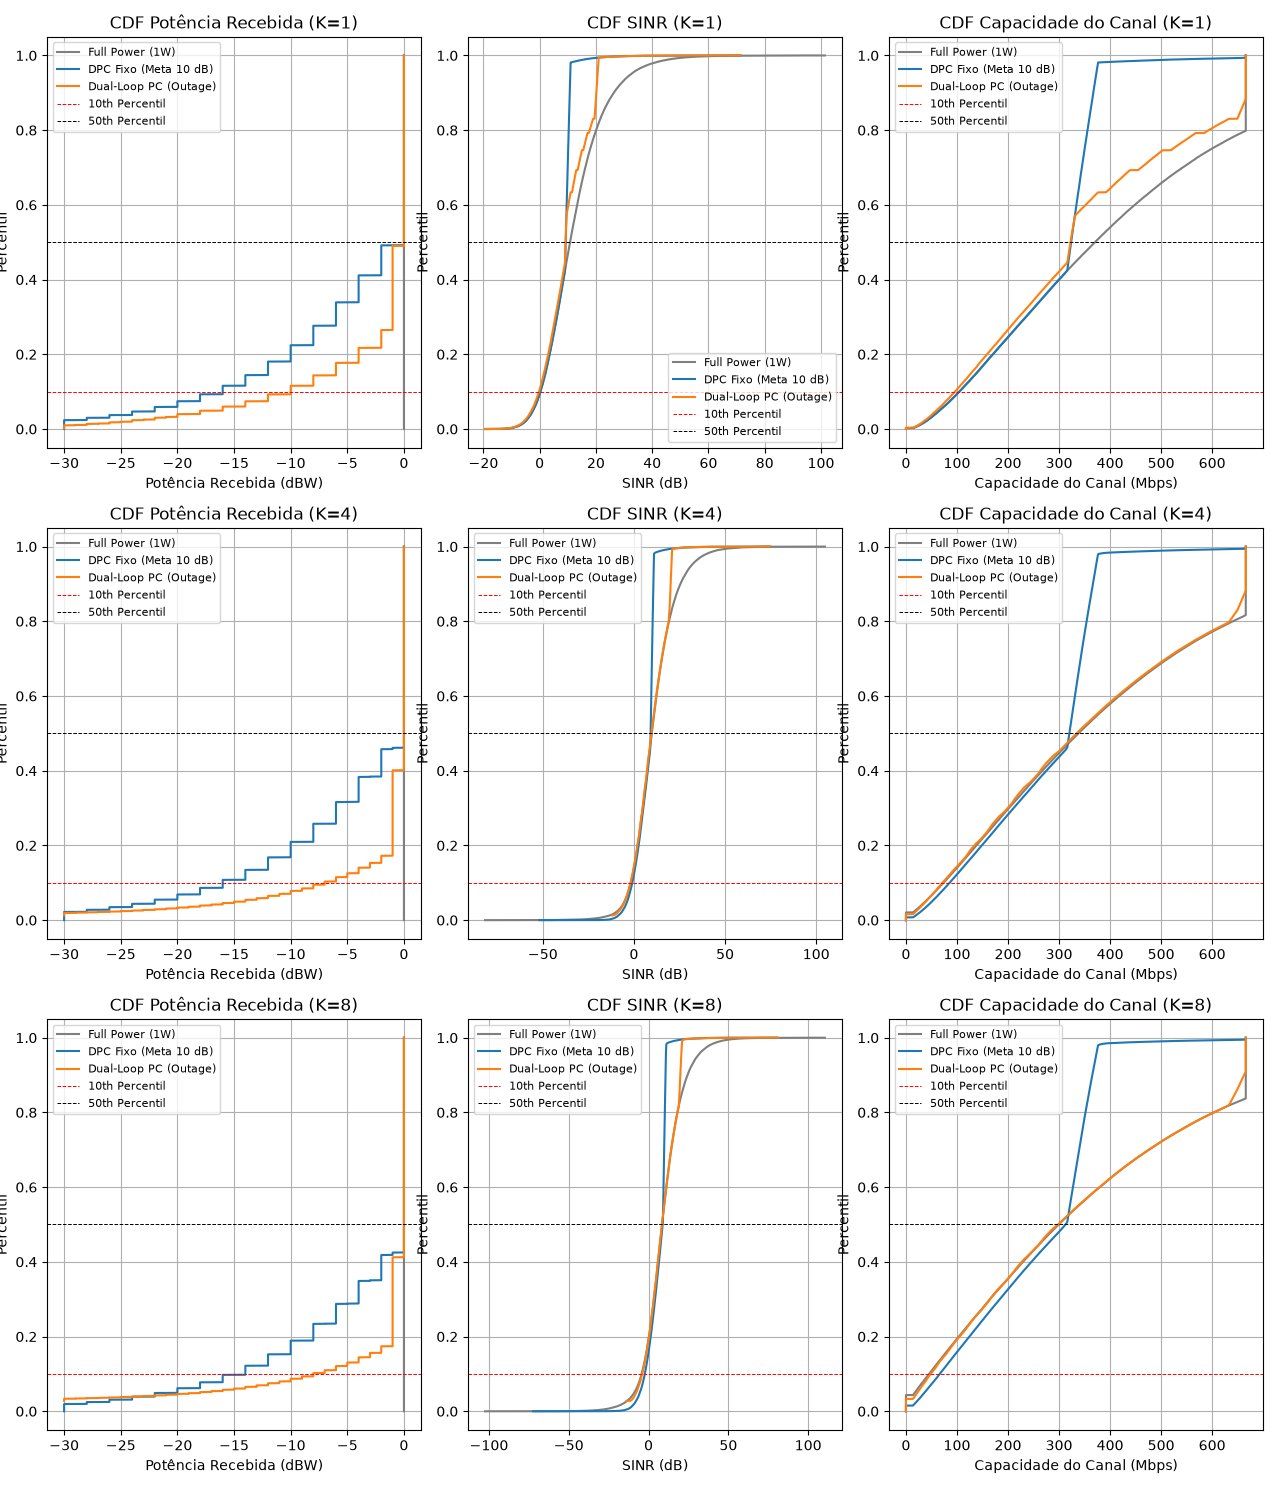
\includegraphics[width=0.98\linewidth]{Imagens/Activity01A.png}
    \caption{CDFs empíricas da Potência Transmitida/Recebida (dBW), SINR (dB) e Capacidade do Canal (Mbps) sob cargas de $K=1$, $K=4$ e $K=8$ UEs.}
    \label{fig:act1_cdfs}
\end{figure}

As curvas da Figura \ref{fig:act1_cdfs} evidenciam a mecânica de funcionamento das três estratégias:
\begin{itemize}
    \item \textbf{CDF de Potência (Coluna Esquerda):} Enquanto a estratégia \textit{Full Power} mantém 100\% dos usuários cravados em $0\text{ dBW}$ ($1\text{ W}$), tanto o \textit{DPC Fixo} quanto o \textit{Dual-Loop PC} apresentam curvas em degraus (efeito dos passos discretos em dB), demonstrando que mais de 50\% dos UEs operam com potências significativamente inferiores à máxima.
    \item \textbf{CDF de SINR (Coluna Central):} No \textit{DPC Fixo} (curva azul), observa-se um degrau vertical abrupto exatamente em $\text{SINR} = 10\text{ dB}$, confirmando que cerca de 60\% a 80\% dos usuários ficam represados nessa meta fixa. Já no \textbf{Dual-Loop PC} (curva laranja), a distribuição acompanha a evolução da capacidade até o degrau vertical de saturação em $+20\text{ dB}$, comprovando o sucesso da negociação ascendente de metas pelo \textit{Outer Loop}.
    \item \textbf{CDF de Capacidade do Canal (Coluna Direita):} Devido ao truncamento físico de modulação em $\gamma_{\max} = 20\text{ dB}$ ($\approx 665.8\text{ Mbps}$ em $100\text{ MHz}$), a curva do \textit{Dual-Loop PC} sobrepõe-se quase perfeitamente à curva de \textit{Full Power} nos percentis superiores, entregando a mesma vazão máxima com consumo energético drasticamente reduzido.
\end{itemize}

% ----------------------------------------------------------- %
\newpage
\section{Atividade 2: Impacto da Mobilidade no Desempenho do \textit{Beamforming}}

A segunda atividade realiza a transição de \textit{snapshots} estáticos de Monte Carlo para uma simulação dinâmica orientada ao tempo (\textit{time-driven simulation}), com resolução temporal física de $dt = 1\text{ ms}$. Avalia-se um cenário onde um único UE equipado com antena omnidirecional atravessa a célula tangencialmente à direção principal (\textit{broadside}) de um AP equipado com um Arranjo Linear Uniforme (ULA) de espaçamento $d = \lambda / 2$.

\subsection{Modelagem Cinemática, ULA e Atraso de Rastreamento (\textit{Update Lag})}

O AP encontra-se posicionado na origem $(0,0)$, com o eixo do arranjo alinhado ao eixo $X$ e a direção de \textit{broadside} ($\theta = 0^\circ$) apontando para o eixo $Y$ positivo. O terminal móvel desloca-se paralelamente ao eixo $X$ com velocidade escalar constante $v$, mantendo uma distância perpendicular fixa $y(t) = D$ em uma janela temporal de $T_{\text{sim}} = 4.0\text{ s}$ centralizada no cruzamento em frente à antena ($x = 0$ em $t = 2.0\text{ s}$):
\begin{equation}
    x(t) = v \cdot \left(t - \frac{T_{\text{sim}}}{2}\right), \quad \theta_{\text{real}}(t) = \arctan\left(\frac{x(t)}{D}\right)
\end{equation}

O ganho direcional normalizado do arranjo ULA com $L$ elementos quando o feixe é apontado para o ângulo estimado $\theta_{\text{tgt}}$ enquanto o terminal se encontra na direção real $\theta_{\text{real}}(t)$ é expresso por:
\begin{equation}
    G_{\text{ULA}}\big(\theta_{\text{real}}(t), \theta_{\text{tgt}}\big) = \frac{1}{L} \left| \sum_{\ell=0}^{L-1} e^{j \pi \ell \left[\sin(\theta_{\text{real}}(t)) - \sin(\theta_{\text{tgt}})\right]} \right|^2
\end{equation}

Na prática, os procedimentos de RRM atualizam os pesos do feixe periodicamente a cada intervalo $\Delta T \in \{100, 50, 10\}\text{ ms}$. Durante os instantes entre atualizações consecutivas, o ângulo alvo $\theta_{\text{tgt}}$ permanece congelado enquanto o veículo avança, gerando um erro angular acumulado por atraso ($\epsilon_{\text{lag}}$) que se soma ao erro de estimação de chegada ($\epsilon_{\text{estimation}}$):
\begin{equation}
    \epsilon_{\text{total}}(t) = \epsilon_{\text{estimation}}(\sigma_\theta) + \epsilon_{\text{lag}}(v, \Delta T)
\end{equation}

Além disso, cada atualização de feixe exige a transmissão de sinais pilotos de treinamento (\textit{beam training overhead} de duração $T_{\text{overhead}}$), reduzindo a fração de tempo disponível para dados úteis e definindo a Eficiência Espectral Líquida (\textit{Net Spectral Efficiency}):
\begin{equation}
    \text{SE}_{\text{líquida}}(t) = \left(1 - \frac{T_{\text{overhead}}}{\Delta T}\right) \log_2\big(1 + \text{SNR}(t)\big)
\end{equation}

\subsection{Dinâmica Temporal: Ganho do Arranjo e Perda por Desalinhamento}

A Figura \ref{fig:act2_time} ilustra a evolução temporal do Ganho do Arranjo (\textit{Array Gain vs. Time}) e da Perda por Desalinhamento (\textit{Beam Misalignment Loss}, dada por $G_{\text{ideal, dB}} - G_{\text{real, dB}}$) para o cenário de rodovia (\textit{Highway}, $v = 120\text{ km/h}$) a uma distância perpendicular de $D = 50\text{ m}$.

\begin{figure}[H]
    \centering
    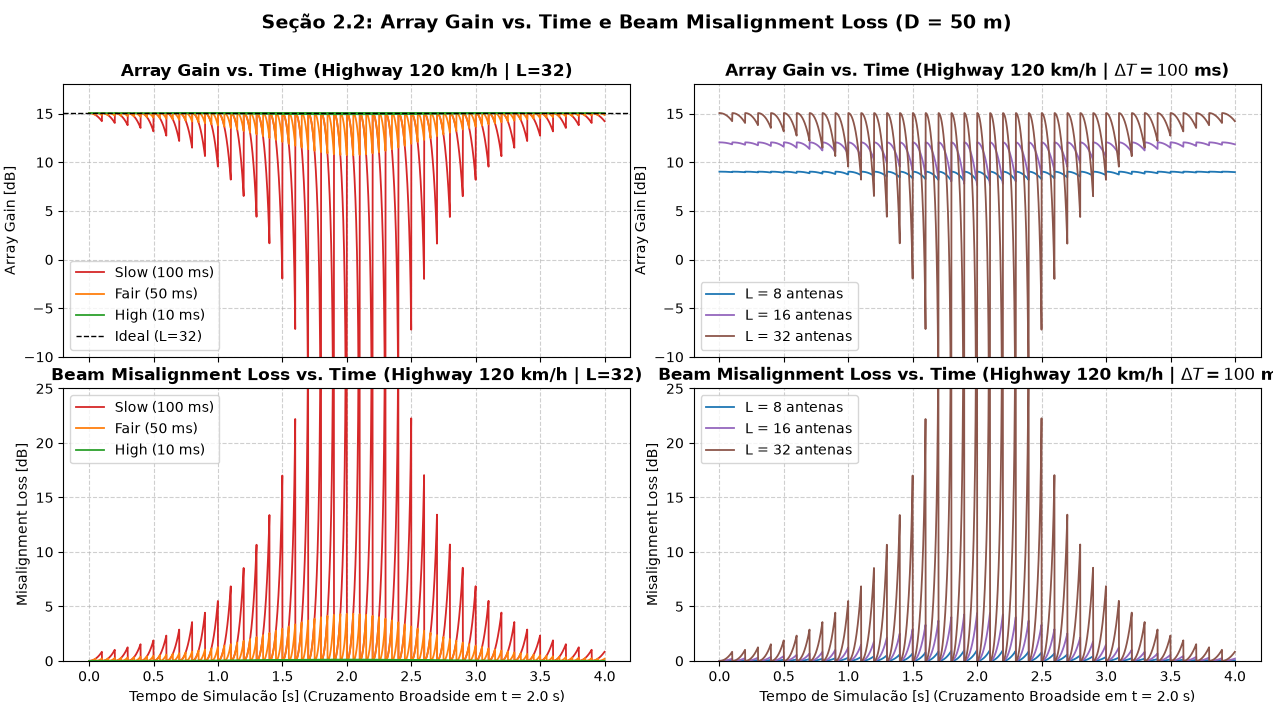
\includegraphics[width=0.98\linewidth]{Imagens/Activity02B.png}
    \caption{Evolução temporal do Ganho do Arranjo (topo) e da Perda por Desalinhamento de Feixe (base) para o perfil \textit{Highway} ($120\text{ km/h}$, $D = 50\text{ m}$): efeito da taxa de atualização $\Delta T$ com $L=32$ (esquerda) e efeito do número de antenas $L$ com $\Delta T = 100\text{ ms}$ (direita).}
    \label{fig:act2_time}
\end{figure}

Da inspeção da Figura \ref{fig:act2_time}, extraem-se três conclusões fundamentais sobre a física de rastreamento de feixe:
\begin{itemize}
    \item \textbf{Padrão "Dente de Serra" (\textit{Sawtooth}) e Velocidade Angular no \textit{Broadside}:} A cada múltiplo de $\Delta T$, o AP reorienta o feixe para a posição atual do veículo, restaurando o ganho ao patamar máximo teórico ($10\log_{10}(L) \approx 15.05\text{ dB}$ para $L=32$) e zerando a perda. À medida que o veículo se desloca durante a janela $\Delta T$, o ganho cai progressivamente. Essa degradação atinge seu ápice exatamente em torno de $t = 2.0\text{ s}$ (passagem pelo \textit{broadside}, $x=0$), onde a velocidade angular $\omega(t) = \frac{d\theta}{dt} = \frac{v \cos^2(\theta)}{D}$ é máxima.
    \item \textbf{Impacto da Taxa de Atualização $\Delta T$ (Coluna Esquerda):} Operando com $L=32$ antenas a $120\text{ km/h}$ ($33.33\text{ m/s}$), uma atualização lenta ($\Delta T = 100\text{ ms}$, curva vermelha) faz com que o veículo percorra $3.33\text{ m}$ sem reajuste de fase. No cruzamento central, esse deslocamento retira o terminal do lóbulo principal e o lança sobre os nulos do fator de arranjo, provocando quedas severas que ultrapassam $25\text{ dB}$ de perda. Ao reduzir o intervalo para $\Delta T = 50\text{ ms}$ (curva laranja), a perda máxima cai para $\approx 4.5\text{ dB}$; já em $\Delta T = 10\text{ ms}$ (curva verde), o rastreamento é praticamente contínuo e a perda torna-se desprezível ($< 0.2\text{ dB}$).
    \item \textbf{Sensibilidade Direcional vs. Tamanho do Arranjo $L$ (Coluna Direita):} Embora o arranjo \textit{Massive MIMO} ($L=32$, curva marrom) proporcione o maior ganho de pico ($15.05\text{ dB}$ contra $12.04\text{ dB}$ de $L=16$ e $9.03\text{ dB}$ de $L=8$), ele possui a menor abertura de meia potência (feixe extremamente estreito). Como consequência, sob $\Delta T = 100\text{ ms}$, o ganho instantâneo de $L=32$ no intervalo central ($1.3\text{ s}$ a $2.7\text{ s}$) colapsa para valores inferiores aos entregues pelos arranjos menores e mais largos ($L=8$ e $L=16$), cuja perda máxima no centro não ultrapassa $\approx 1.0\text{ dB}$ e $\approx 4.5\text{ dB}$, respectivamente.
\end{itemize}

\subsection{Impacto dos Perfis de Velocidade e da Distância Tangencial ao AP}

A Figura \ref{fig:act2_vel_dist} isola o efeito da velocidade linear $v \in \{3, 50, 120\}\text{ km/h}$ (a uma distância fixa $D = 50\text{ m}$) e o efeito da variação da distância perpendicular $D \in \{25, 75, 150\}\text{ m}$ (fixando o perfil urbano de $50\text{ km/h}$) para a configuração mais diretiva ($L=32$, $\Delta T = 100\text{ ms}$).

\begin{figure}[H]
    \centering
    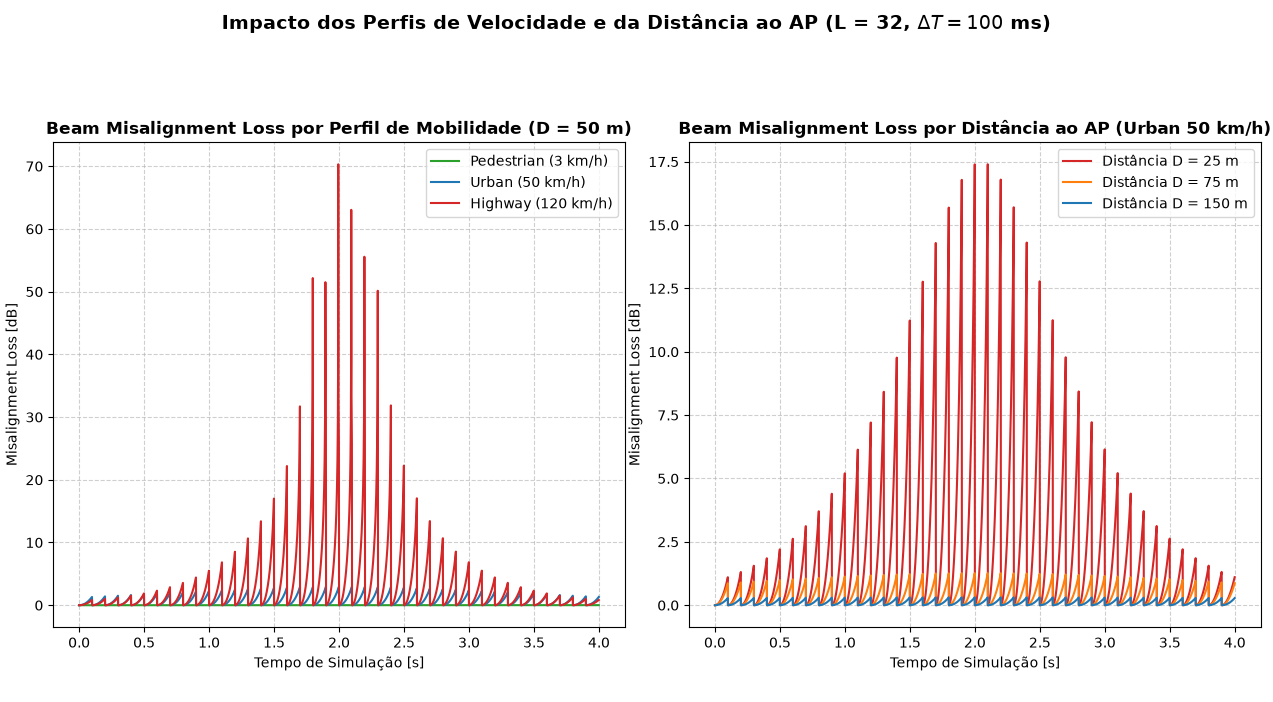
\includegraphics[width=0.98\linewidth]{Imagens/Activity02C.png}
    \caption{Perda por desalinhamento de feixe (\textit{Beam Misalignment Loss}) para $L=32$ e $\Delta T = 100\text{ ms}$: comparação entre os três perfis de mobilidade a $D=50\text{ m}$ (esquerda) e variação da distância tangencial $D \in \{25, 75, 150\}\text{ m}$ a $50\text{ km/h}$ (direita).}
    \label{fig:act2_vel_dist}
\end{figure}

Os resultados da Figura \ref{fig:act2_vel_dist} demonstram que:
\begin{itemize}
    \item \textbf{Perfis de Velocidade (Esquerda):} No perfil \textit{Pedestrian} ($3\text{ km/h}$, curva verde), o deslocamento de $8.3\text{ cm}$ por janela de $100\text{ ms}$ é insuficiente para descolar o usuário do centro do lóbulo principal, resultando em $0.00\text{ dB}$ de perda durante todo o trajeto. No perfil \textit{Urban} ($50\text{ km/h}$, curva azul), surgem oscilações moderadas na passagem pelo \textit{broadside} com picos de $\approx 3.2\text{ dB}$. Já no perfil \textit{Highway} ($120\text{ km/h}$, curva vermelha), a passagem pelos nulos profundos do diagrama de radiação de 32 elementos gera picos instantâneos de atenuação de até $70\text{ dB}$.
    \item \textbf{Geometria da Distância ao AP (Direita):} Quando o veículo passa muito próximo ao AP ($D = 25\text{ m}$, curva vermelha), o raio de giro é curto e a velocidade angular máxima ($\omega_{\max} = v/D$) dobra em relação a $D = 50\text{ m}$, elevando os picos de perda por desalinhamento para $17.5\text{ dB}$ mesmo em velocidade urbana ($50\text{ km/h}$). À medida que o usuário se afasta para o meio ($D = 75\text{ m}$, curva laranja) e para a borda da célula ($D = 150\text{ m}$, curva azul), a variação angular suaviza-se drasticamente, reduzindo os picos de desalinhamento para valores inferiores a $1.4\text{ dB}$ e $0.4\text{ dB}$, respectivamente. Assim, usuários próximos ao AP possuem excelente ganho de percurso, mas exigem rastreamento angular rápido; usuários de borda sofrem alta perda de percurso por distância, mas demandam baixíssima frequência de atualização de feixe.
\end{itemize}

\subsection{\textit{Trade-off} entre Taxa de Atualização e Eficiência Espectral Líquida}

A Tabela \ref{tab:act2_full} e a Figura \ref{fig:act2_tradeoff} consolidam os resultados numéricos das 27 combinações paramétricas exigidas na Seção 2.2 ($D = 50\text{ m}$), confrontando a Perda Média por Desalinhamento (em dB) com a Eficiência Espectral Líquida Média (em bps/Hz).

\begin{table}[H]
    \centering
    \caption{Resultados Consolidados da Seção 2.2: Perda Média por Desalinhamento e Eficiência Espectral Líquida ($D = 50\text{ m}$, $dt = 1\text{ ms}$)}
    \vspace{4pt}
    \resizebox{0.92\textwidth}{!}{
    \begin{tabular}{l|c|c|cc}
        \toprule
        \textbf{Perfil de Mobilidade} & \textbf{Antenas ($L$)} & \textbf{Taxa de Atualização ($\Delta T$)} & \textbf{Perda Média (dB)} & \textbf{SE Líquida (bps/Hz)} \\
        \midrule
        \multirow{9}{*}{Pedestrian ($3\text{ km/h}$)}
        & 8  & Slow ($100\text{ ms}$) & 0.00 & \textbf{6.90} \\
        & 8  & Fair ($50\text{ ms}$)  & 0.00 & 6.80 \\
        & 8  & High ($10\text{ ms}$)  & 0.00 & 5.96 \\
        \cmidrule{2-5}
        & 16 & Slow ($100\text{ ms}$) & 0.00 & \textbf{7.88} \\
        & 16 & Fair ($50\text{ ms}$)  & 0.00 & 7.76 \\
        & 16 & High ($10\text{ ms}$)  & 0.00 & 6.80 \\
        \cmidrule{2-5}
        & 32 & Slow ($100\text{ ms}$) & 0.00 & \textbf{8.87} \\
        & 32 & Fair ($50\text{ ms}$)  & 0.00 & 8.73 \\
        & 32 & High ($10\text{ ms}$)  & 0.00 & 7.65 \\
        \midrule
        \multirow{9}{*}{Urban ($50\text{ km/h}$)}
        & 8  & Slow ($100\text{ ms}$) & 0.04 & \textbf{6.63} \\
        & 8  & Fair ($50\text{ ms}$)  & 0.01 & 6.54 \\
        & 8  & High ($10\text{ ms}$)  & 0.00 & 5.73 \\
        \cmidrule{2-5}
        & 16 & Slow ($100\text{ ms}$) & 0.18 & \textbf{7.56} \\
        & 16 & Fair ($50\text{ ms}$)  & 0.04 & 7.49 \\
        & 16 & High ($10\text{ ms}$)  & 0.00 & 6.57 \\
        \cmidrule{2-5}
        & 32 & Slow ($100\text{ ms}$) & 0.74 & 8.36 \\
        & 32 & Fair ($50\text{ ms}$)  & 0.18 & \textbf{8.41} \\
        & 32 & High ($10\text{ ms}$)  & 0.01 & 7.42 \\
        \midrule
        \multirow{9}{*}{Highway ($120\text{ km/h}$)}
        & 8  & Slow ($100\text{ ms}$) & 0.14 & \textbf{5.71} \\
        & 8  & Fair ($50\text{ ms}$)  & 0.03 & 5.65 \\
        & 8  & High ($10\text{ ms}$)  & 0.00 & 4.96 \\
        \cmidrule{2-5}
        & 16 & Slow ($100\text{ ms}$) & 0.59 & 6.53 \\
        & 16 & Fair ($50\text{ ms}$)  & 0.14 & \textbf{6.58} \\
        & 16 & High ($10\text{ ms}$)  & 0.00 & 5.80 \\
        \cmidrule{2-5}
        & 32 & Slow ($100\text{ ms}$) & 3.08 & 6.75 \\
        & 32 & Fair ($50\text{ ms}$)  & 0.59 & \textbf{7.39} \\
        & 32 & High ($10\text{ ms}$)  & 0.02 & 6.64 \\
        \bottomrule
    \end{tabular}}
    \label{tab:act2_full}
\end{table}

\begin{figure}[H]
    \centering
    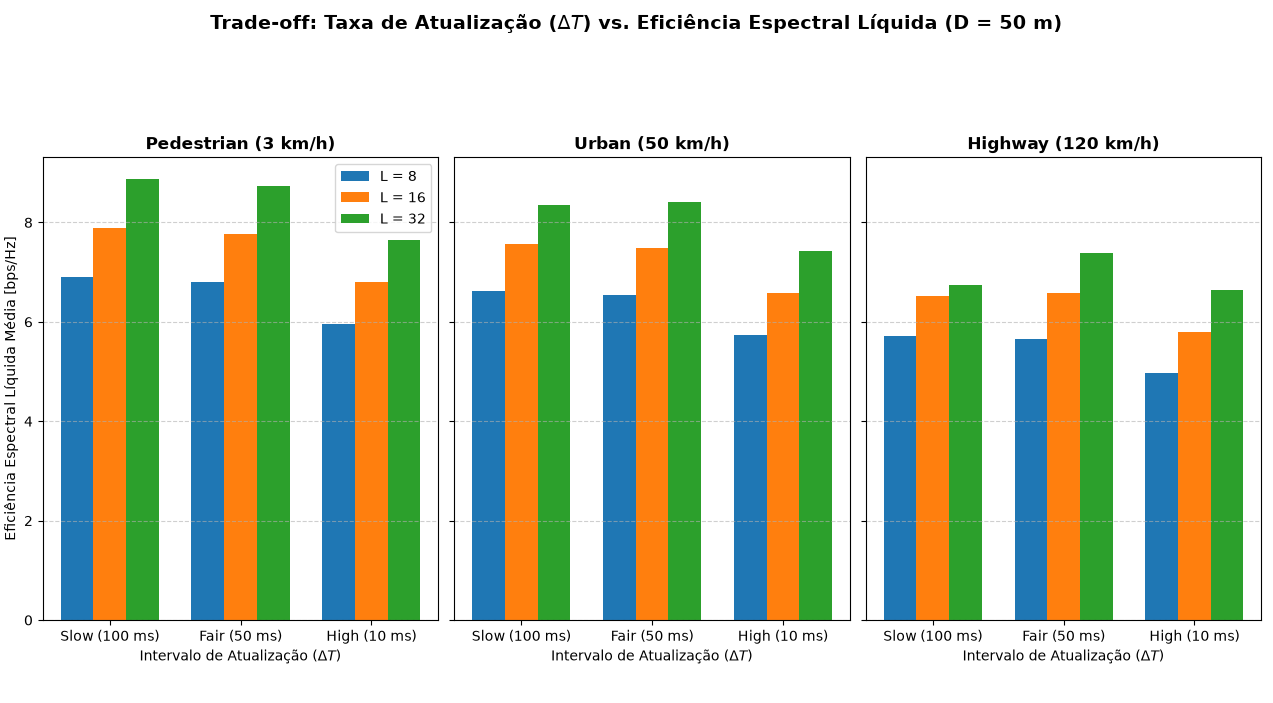
\includegraphics[width=0.98\linewidth]{Imagens/Activity02A.png}
    \caption{\textit{Trade-off} entre o intervalo de atualização de feixe ($\Delta T$) e a Eficiência Espectral Líquida Média para os três perfis de mobilidade e configurações de ULA ($L \in \{8, 16, 32\}$).}
    \label{fig:act2_tradeoff}
\end{figure}

A avaliação conjunta da Tabela \ref{tab:act2_full} e da Figura \ref{fig:act2_tradeoff} explicita o compromisso fundamental entre a precisão de apontamento do feixe e o custo de sinalização (\textit{overhead}) de RRM:

\begin{itemize}
    \item \textbf{Regime Estático / Baixa Mobilidade (\textit{Pedestrian} — $3\text{ km/h}$):} Como a perda média por desalinhamento é nula ($0.00\text{ dB}$) em qualquer configuração, reduzir $\Delta T$ de $100\text{ ms}$ para $10\text{ ms}$ degrada a eficiência espectral líquida de $8.87\text{ bps/Hz}$ para $7.65\text{ bps/Hz}$ em $L=32$ (queda de $13.8\%$). Nesse regime, atualizações frequentes apenas desperdiçam recursos temporais do canal com envio de pilotos redundantes, tornando $\Delta T = 100\text{ ms}$ (\textit{Slow}) a escolha ótima para todos os tamanhos de arranjo.
    \item \textbf{Regime Urbano (\textit{Urban} — $50\text{ km/h}$):} Para feixes mais largos ($L=8$ e $L=16$), a perda angular em $\Delta T = 100\text{ ms}$ ainda é pequena ($0.04\text{ dB}$ e $0.18\text{ dB}$), mantendo a taxa lenta como ótima ($6.63$ e $7.56\text{ bps/Hz}$). Entretanto, para \textit{Massive MIMO} ($L=32$), a perda média em $100\text{ ms}$ sobe para $0.74\text{ dB}$, fazendo com que a taxa intermediária $\Delta T = 50\text{ ms}$ (\textit{Fair}) reduza a perda para $0.18\text{ dB}$ e supere a taxa lenta em eficiência líquida ($8.41\text{ bps/Hz}$ contra $8.36\text{ bps/Hz}$).
    \item \textbf{Regime de Alta Mobilidade (\textit{Highway} — $120\text{ km/h}$):} Sob atualização lenta ($\Delta T = 100\text{ ms}$), o severo desalinhamento médio de $3.08\text{ dB}$ em $L=32$ derruba sua eficiência líquida para $6.75\text{ bps/Hz}$, quase anulando o ganho espacial do \textit{Massive MIMO} frente ao arranjo de $L=16$ ($6.53\text{ bps/Hz}$). Ao adotar a atualização moderada $\Delta T = 50\text{ ms}$ (\textit{Fair}), a perda média em $L=32$ despenca para $0.59\text{ dB}$ e a eficiência espectral líquida salta para o valor ótimo de $\mathbf{7.39\text{ bps/Hz}}$ (e $\mathbf{6.58\text{ bps/Hz}}$ para $L=16$). Por outro lado, forçar $\Delta T = 10\text{ ms}$ (\textit{High}), embora elimine quase totalmente o desalinhamento ($0.02\text{ dB}$), penaliza excessivamente o termo $(1 - T_{\text{overhead}}/\Delta T)$, derrubando a eficiência líquida para $6.64\text{ bps/Hz}$.
\end{itemize}

Conclui-se que sistemas \textit{Massive MIMO} exigem mecanismos de RRM sensíveis ao contexto cinemático do usuário: a periodicidade de treinamento de feixes $\Delta T$ deve ser adaptada dinamicamente em função da velocidade angular estimada ($\omega \propto v/D$) e da largura de feixe do arranjo ($L$), maximizando a vazão líquida entregue ao terminal móvel.

\end{document}